\RequirePackage[T1]{fontenc}
\documentclass[conference]{IEEEtran}

\usepackage{amsmath,amssymb}
\usepackage{array}
\usepackage{balance}
\usepackage{booktabs}
\usepackage{cite}
\usepackage{graphicx}
\usepackage{url}

\graphicspath{{figures/}}
\interdisplaylinepenalty=2500
\setlength{\floatsep}{6pt plus 1pt minus 2pt}
\setlength{\textfloatsep}{8pt plus 1pt minus 2pt}
\setlength{\dblfloatsep}{6pt plus 1pt minus 2pt}
\setlength{\dbltextfloatsep}{8pt plus 1pt minus 2pt}
\hyphenation{ARIMA GARCH EGARCH FIGARCH APARCH LSTM HistoricalMean RollingVol}

\newcolumntype{L}[1]{>{\raggedright\arraybackslash}p{#1}}
\newcommand{\best}[1]{\textbf{#1}}
\newcommand{\takeaway}[1]{\textbf{#1}}

\begin{document}

\title{Modeling and Forecasting VN-Index Volatility: A Financial Econometric Evaluation of GARCH-Family, HAR, Neural, and Hybrid Approaches}

\author{
\IEEEauthorblockN{Tran Anh Tuan - 1120399 - DSEB 65B - NEU}
\IEEEauthorblockA{Course: Time Series}
}

\maketitle

\begin{abstract}
This paper studies one-step-ahead daily VN-Index volatility forecasting using CafeF OHLC and trading-activity data. The target is next-day squared percentage log return, and all primary forecasts are evaluated on a unified out-of-sample window of 726 common target dates from 2023-02-07 to 2025-12-31. The study compares historical and rolling variance baselines, EWMA/RiskMetrics, HAR-type models, GARCH(1,1), ARIMA-GARCH, validation-selected GARCH-family specifications, LSTM, hybrid neural forecasts, calibration, and forecast combinations. Descriptive diagnostics show negatively skewed, heavy-tailed returns, and ARCH-LM tests strongly reject homoskedasticity, motivating conditional-variance models. On the corrected common window, AdvGARCH-BestAsymmetric obtains QLIKE 1.0214, the primary validation-selected AdvGARCH-BestQLIKE obtains 1.0229, HAR-Parkinson obtains 1.0294, and GARCH(1,1) obtains 1.0529. The evidence supports a conservative class-level conclusion: selected GARCH-family specifications and HAR-Parkinson form the strongest group, while the implemented neural and hybrid approaches do not robustly outperform these econometric benchmarks in this modest daily-data setting. Risk diagnostics qualify the average-loss ranking. Under a common-Normal variance-to-VaR mapping, GARCH(1,1) has 15 one-percent violations out of 726 observations, against 7.26 expected, with Kupiec \(p=0.0116\). Thus good QLIKE does not by itself guarantee strict-tail calibration.
\end{abstract}

\begin{IEEEkeywords}
VN-Index, volatility forecasting, GARCH, EGARCH, LSTM, hybrid forecasting, QLIKE, VaR backtesting, range-based volatility.
\end{IEEEkeywords}

\section{Introduction}

Volatility forecasting is a practical market-risk problem. For an equity index, a one-step-ahead conditional-variance forecast summarizes the expected scale of the next return shock and feeds into risk limits, margin decisions, portfolio monitoring, and Value-at-Risk (VaR). A model can look accurate on average while still being too low when volatility spikes, which is exactly when risk forecasts matter most.

The VN-Index is a useful Vietnamese equity-market case study. It is an emerging-market index with visible volatility clustering, sharp drawdowns, and changing trading conditions, but without the routine high-frequency realized-volatility data often used in developed-market volatility studies. Daily open, high, low, close, volume, and trading-value data therefore create a realistic empirical setting: forecasts must be made from daily information, and latent volatility must be evaluated through imperfect observable proxies.

This paper is positioned as a reproducible empirical financial econometrics study, not as a new forecasting algorithm. The main question is whether daily VN-Index volatility can be forecast reliably using standard financial econometric models, and whether neural or hybrid alternatives provide robust gains once model selection, proxy uncertainty, and tail-risk diagnostics are considered. The main target is next-day squared percentage log return, and the primary comparison uses a leakage-safe common test window with identical dates for all primary models.

The contribution is fivefold:
\begin{enumerate}
\item A reproducible, leakage-safe out-of-sample comparison of daily VN-Index volatility forecasts on a corrected 745-observation common test window.
\item Econometric evidence on VN-Index return non-normality, volatility clustering, ARCH effects, and conditional-variance persistence.
\item A validation-based comparison of EWMA, HAR, GARCH-family, corrected-context neural, hybrid, calibrated, and combined volatility forecasts.
\item Proxy-robustness, spike-underprediction, refit-robustness, common-Normal VaR/ES, and model-specific Normal GARCH VaR/ES diagnostics that connect average forecast accuracy to practical risk interpretation.
\item A controlled validation-frozen regime-aware combination that tests whether corrected neural forecasts add useful high-volatility information without test-period tuning.
\end{enumerate}

The verified evidence supports a conservative conclusion. Selected GARCH-family specifications and HAR-Parkinson form the strongest group of daily VN-Index volatility forecasts under the unified common-window protocol. The results are economically consistent with persistent conditional variance and useful OHLC range information. The implemented neural and hybrid forecasts may contain complementary information, but they do not robustly dominate the strongest econometric benchmarks. Tail-risk diagnostics further show that good average QLIKE does not automatically imply adequate one-percent VaR coverage under a common-Normal mapping.

\section{Related Work}

ARCH and GARCH models provide the classical foundation for conditional volatility forecasting. Engle introduced ARCH to model time-varying conditional variance, and Bollerslev generalized the recursion to include lagged conditional variance \cite{engle1982arch,bollerslev1986garch}. The empirical appeal of GARCH(1,1) is not only parsimony. Large-scale forecast comparisons have shown that it can be difficult to beat in practical volatility forecasting applications \cite{hansen2005forecast}.

Mean dynamics are often modeled before conditional variance. The Box-Jenkins ARIMA framework captures serial dependence in univariate time series \cite{box2015time}. In financial returns, the conditional mean is usually small relative to the conditional variance, but an ARMA or ARIMA mean model can still be paired with GARCH to test whether residual variance forecasts improve after filtering predictable mean components.

GARCH-family extensions address stylized features that a symmetric GARCH(1,1) recursion may miss. EGARCH models allow asymmetric volatility responses and avoid some positivity restrictions \cite{nelson1991egarch}. GJR-type models capture sign-dependent shock effects \cite{glosten1993gjr}. APARCH and FIGARCH specifications allow richer power transformations and long-memory volatility dynamics \cite{ding1993aparch,baillie1996figarch}. These extensions motivate the broad specification search evaluated in this paper.

Neural sequence models offer a different forecasting premise. LSTM networks were designed to learn long-range sequential dependencies through gated recurrent states \cite{hochreiter1997lstm}. In volatility forecasting, LSTMs can use lagged returns, volume, rolling volatility, and econometric forecasts as supervised features. Hybrid econometric-neural designs are therefore useful empirical candidates, but their performance must be judged against strong volatility-specific baselines rather than against weak naive alternatives.

Forecast evaluation is central because latent volatility is not directly observed. Squared daily returns are available and simple, but they are noisy proxies for conditional variance. QLIKE is widely used because it remains attractive when forecast comparisons rely on imperfect volatility proxies and because it evaluates forecasts on the variance scale \cite{patton2011volatility}. High-frequency realized volatility can provide richer targets when intraday data are available \cite{andersen2003realized}, but daily OHLC estimators are also useful. Parkinson, Garman-Klass, Rogers-Satchell, and Yang-Zhang estimators exploit high, low, open, and close information to obtain alternative volatility proxies \cite{parkinson1980extreme,garman1980estimation,rogers1991estimating,yang2000drift}.

Statistical forecast comparisons require care when many models are examined. Diebold-Mariano tests compare predictive accuracy under a specified loss difference process \cite{diebold1995predictive}. Holm correction controls family-wise error rates across multiple tests \cite{holm1979sequential}. The model confidence set (MCS) framework provides a complementary way to identify a set of models not statistically eliminated under a loss criterion \cite{hansen2011mcs}. VaR backtesting adds a risk-management view through unconditional and conditional coverage tests \cite{kupiec1995var,christoffersen1998interval}.

\section{Data and Forecasting Target}

\subsection{Daily VN-Index Data}

The empirical sample uses CafeF VNINDEX daily observations from 2010 through 2025. The cleaned data include open, high, low, close, matched trading volume, and matched trading value. Table~\ref{tab:data-splits} reports the chronological splits. The model-ready sample contains 3968 rows from 2010-02-01 to 2025-12-30 after lagged-return, rolling-volatility, and next-day-target requirements are imposed.

\begin{table}[!t]
\centering
\caption{Chronological data splits and common evaluation window. The common-window comparison aligns all original forecasts on 726 target dates from 2023-02-07 to 2025-12-31.}
\label{tab:data-splits}
\scriptsize
\setlength{\tabcolsep}{3pt}
\begin{tabular}{@{}l r L{0.31\columnwidth} L{0.31\columnwidth}@{}}
\toprule
Dataset & Rows & Origin date range & Target date range \\
\midrule
Prepared full & 3989 & 2010-01-04 to 2025-12-31 & 2010-01-05 to 2025-12-31 \\
Model-ready & 3968 & 2010-02-01 to 2025-12-30 & 2010-02-02 to 2025-12-31 \\
Train & 2471 & 2010-02-01 to 2019-12-30 & 2010-02-02 to 2019-12-31 \\
Validation & 750 & 2020-01-02 to 2022-12-29 & 2020-01-03 to 2022-12-30 \\
Test & 745 & 2023-01-03 to 2025-12-30 & 2023-01-04 to 2025-12-31 \\
Common test & 726 & 2023-02-06 to 2025-12-30 & 2023-02-07 to 2025-12-31 \\
\bottomrule
\end{tabular}
\end{table}


The experimental split is chronological. Training observations end in 2019, validation covers 2020--2022, and the test period begins in 2023. The original common-window comparison uses 726 aligned test observations with target dates from 2023-02-07 to 2025-12-31, so every original model is evaluated on identical forecast origins and labels.

\subsection{Squared-Return Target}

Let \(C_t\) denote the VN-Index close on trading day \(t\). Percentage log return is
\begin{equation}
r_t = 100 \log\left(\frac{C_t}{C_{t-1}}\right),
\end{equation}
and the daily squared-return variance proxy is
\begin{equation}
v_t = r_t^2.
\end{equation}
The supervised one-step target is
\begin{equation}
y_t = v_{t+1}=r_{t+1}^{2}.
\end{equation}
Thus a forecast issued at origin date \(t\) uses information available through \(t\) to predict the target date \(t+1\).

Squared daily return is observable and convenient, but it is a noisy volatility proxy. A single daily return can be small even when intraday variation is high, and a single jump can dominate the proxy. This motivates QLIKE-based evaluation and robustness checks with OHLC range-based volatility proxies.

\begin{figure}[!t]
\centering
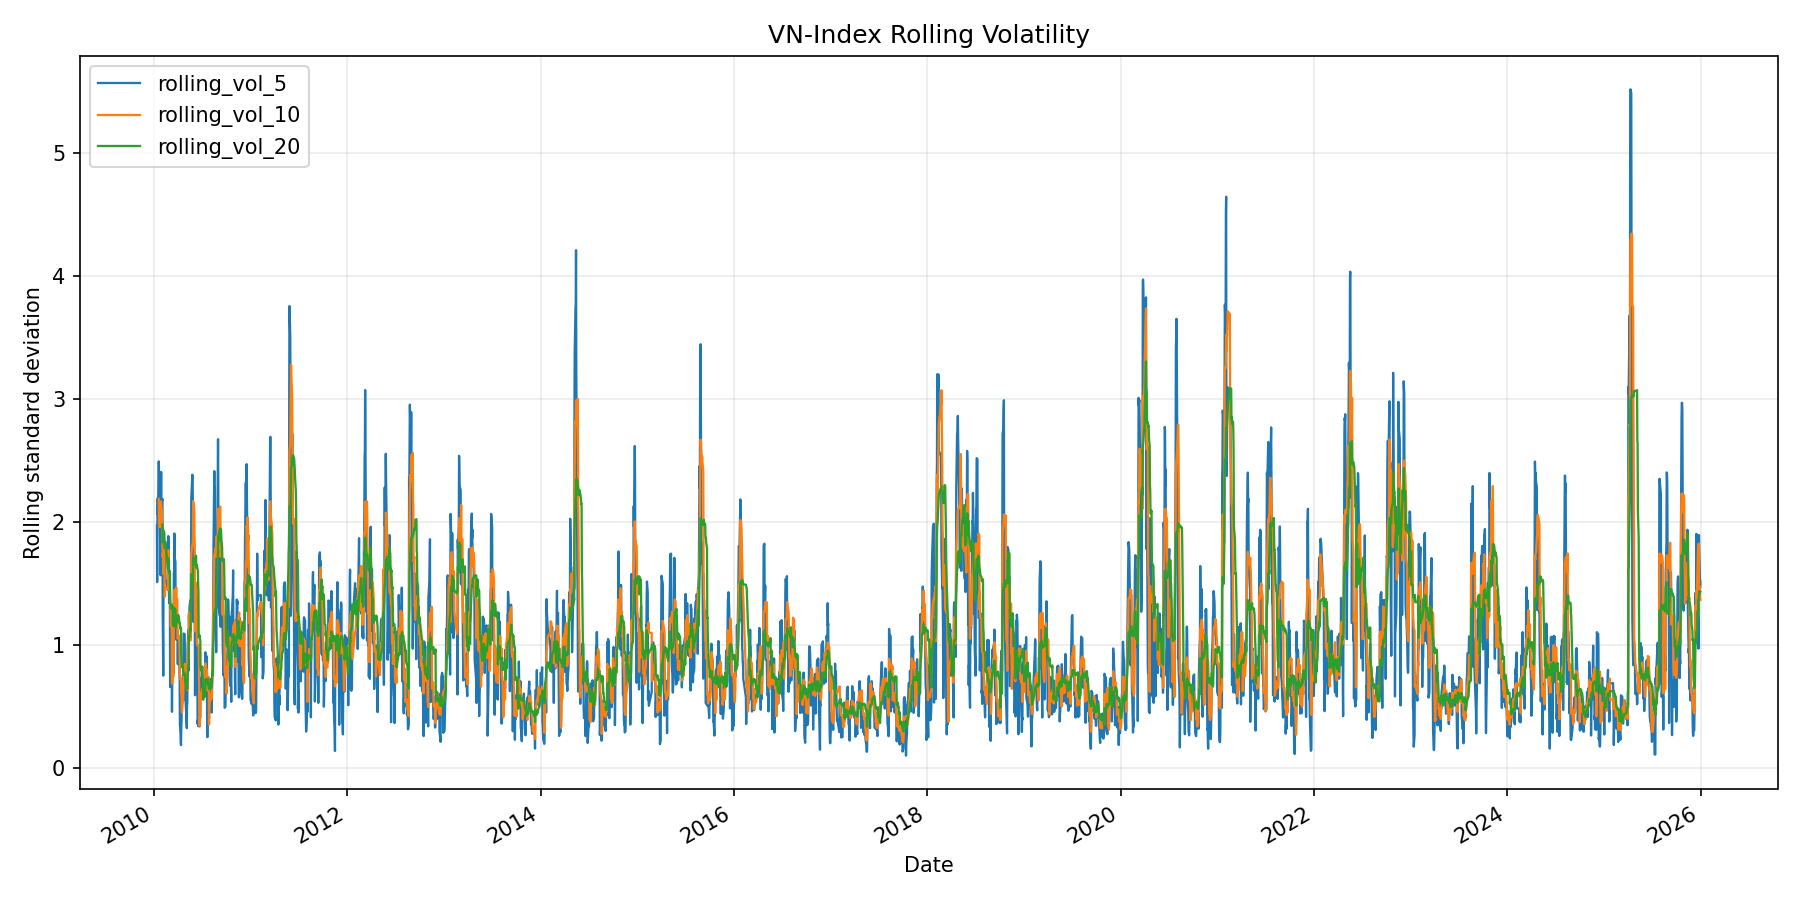
\includegraphics[width=\columnwidth]{fig_rolling_volatility.png}
\caption{Rolling VN-Index volatility changes materially across the sample, motivating conditional-variance models rather than constant-variance forecasts.}
\label{fig:rolling-vol}
\end{figure}

\subsection{OHLC Volatility Proxies}

The proxy robustness analysis constructs seven volatility proxies from the cleaned OHLC sample: close-to-close squared return, Parkinson, Garman-Klass, Rogers-Satchell, and Yang-Zhang rolling proxies over 5, 10, and 20 days. Valid observations range from 3969 for Yang-Zhang 20-day to 3984 for Yang-Zhang 5-day. Correlations with the squared-return proxy are moderate or low: 0.654 for Parkinson, 0.488 for Garman-Klass, 0.345 for Rogers-Satchell, 0.418 for Yang-Zhang 5-day, 0.361 for Yang-Zhang 10-day, and 0.274 for Yang-Zhang 20-day. These values confirm that proxy choice can affect model rankings.

\begin{figure}[!t]
\centering
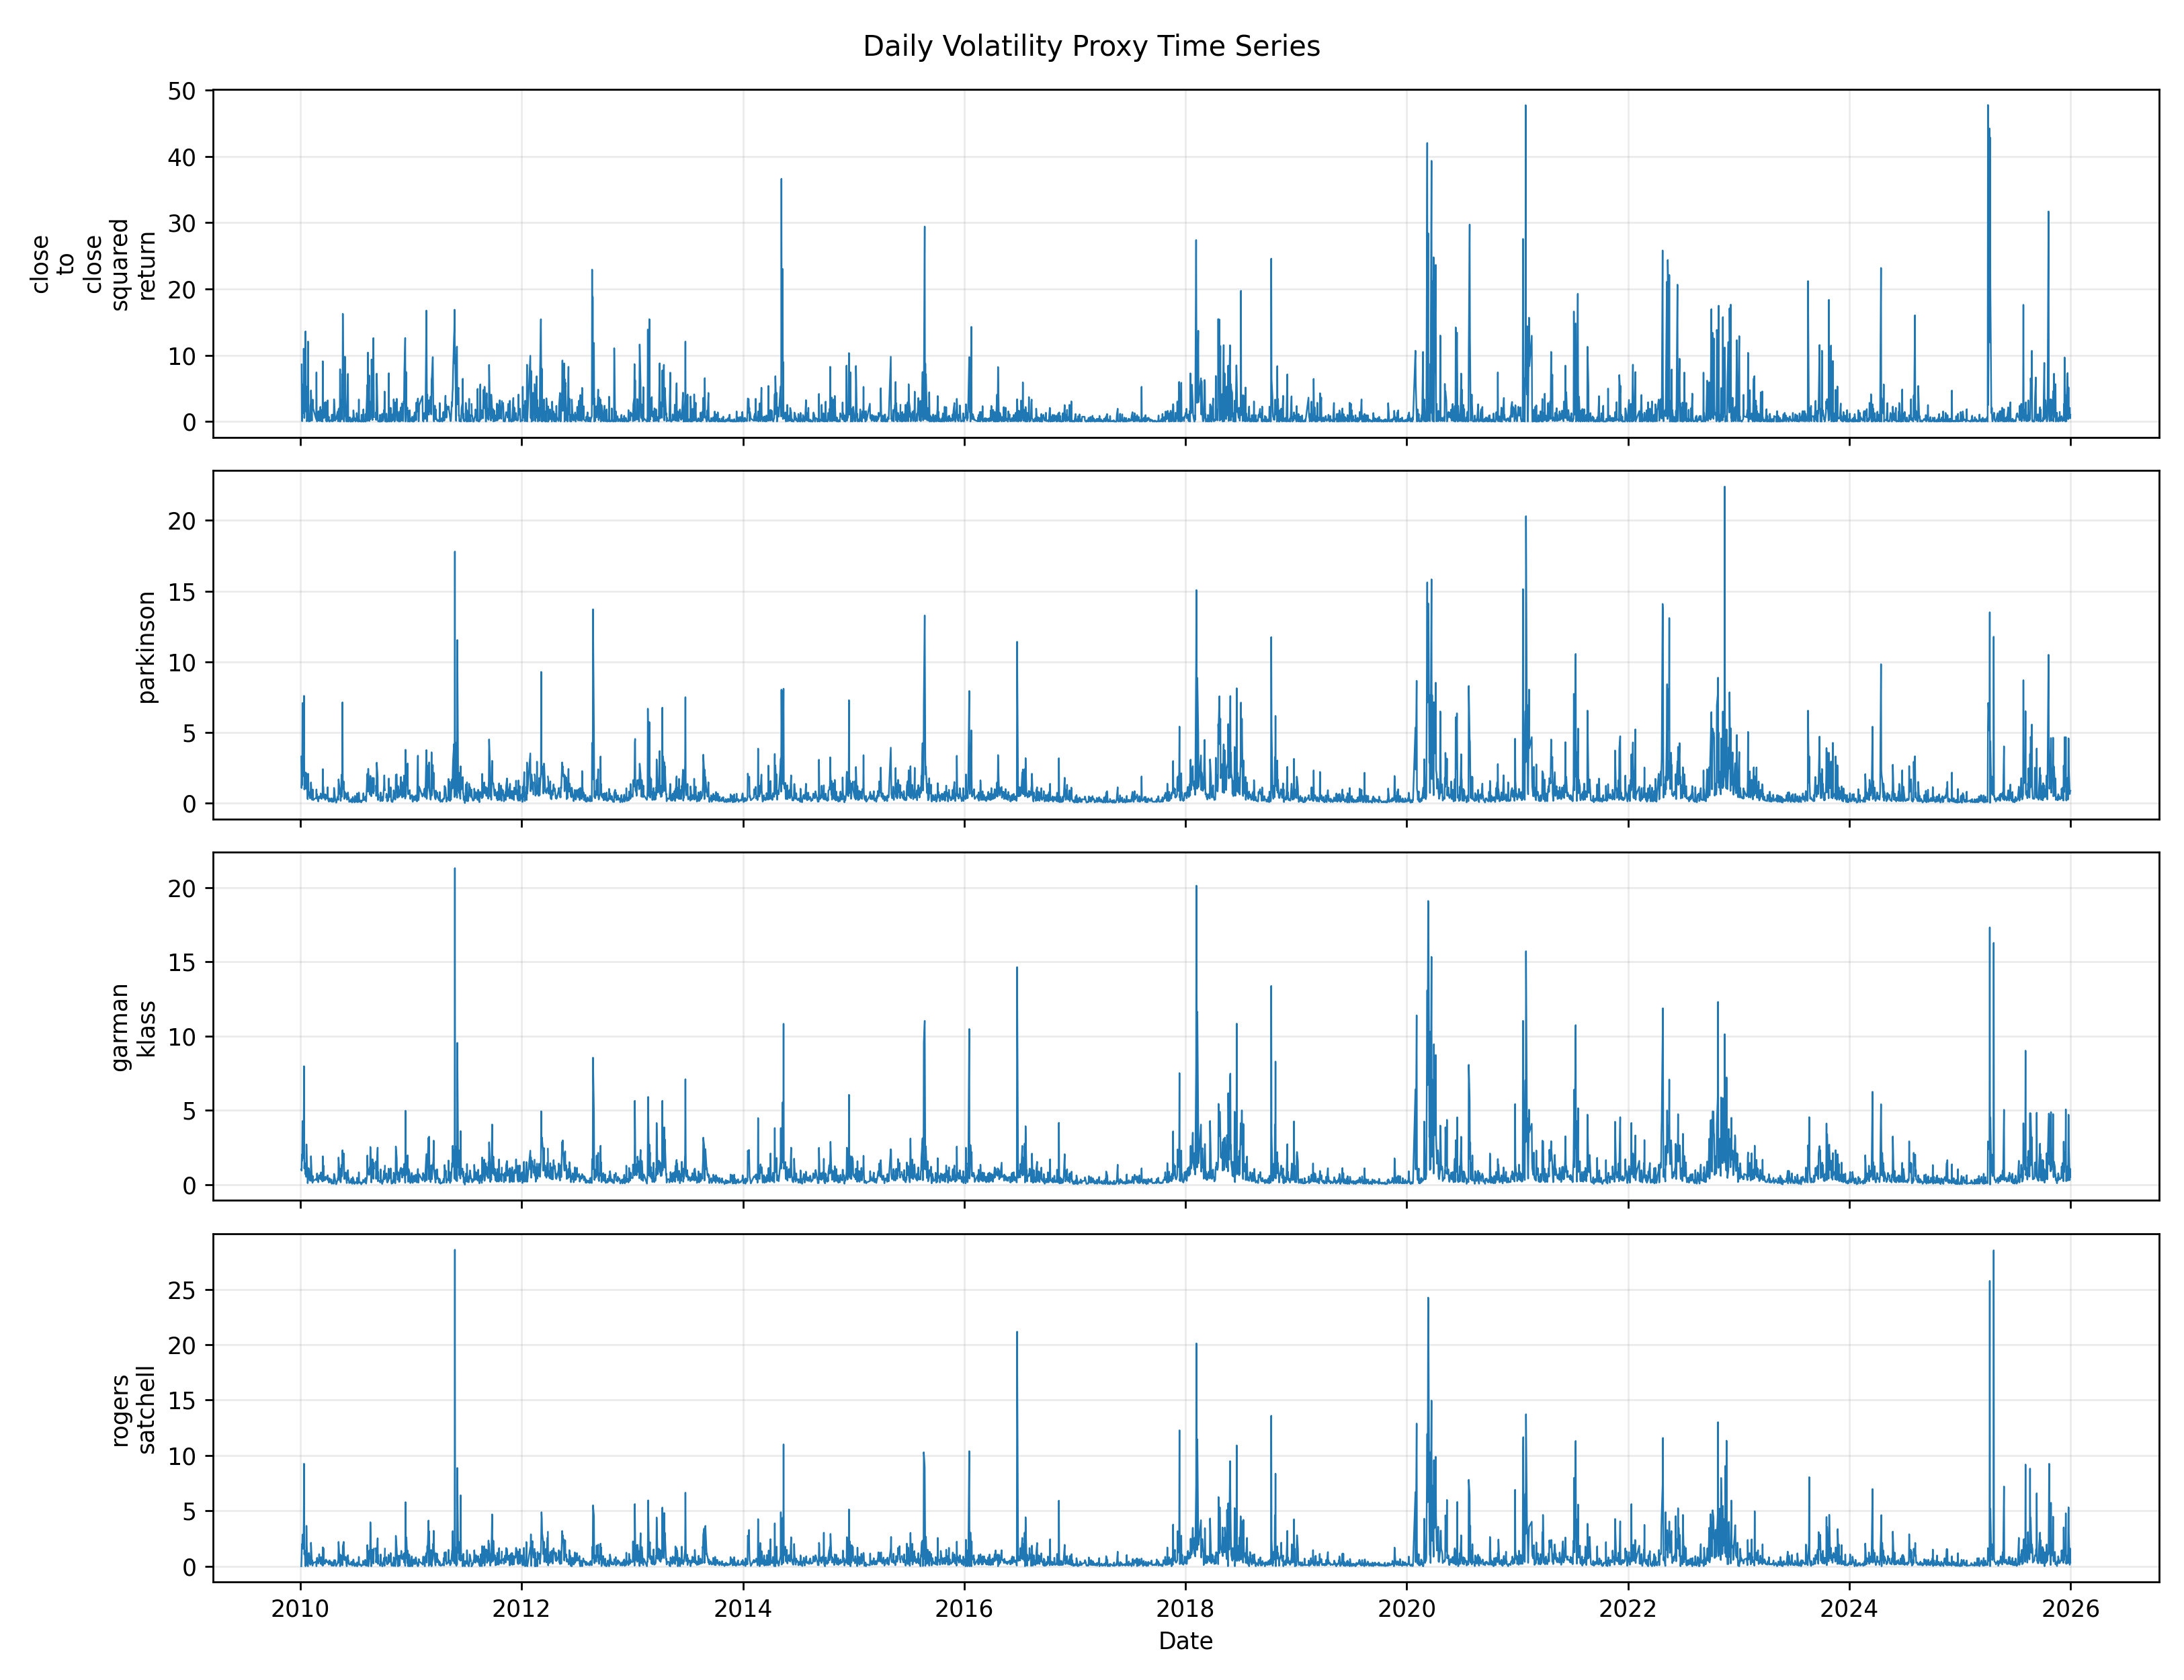
\includegraphics[width=\columnwidth]{fig_volatility_proxy_timeseries.png}
\caption{Alternative volatility proxies have different smoothness and scale, so robustness analysis must distinguish directional conclusions from exact ranking stability.}
\label{fig:proxy-series}
\end{figure}

\section{Models}

\subsection{Baselines}

The historical mean baseline predicts the training-sample average variance. Rolling baselines use 5-, 10-, and 20-day trailing return volatility, squared to produce variance forecasts. These simple baselines are important because volatility is persistent and recent realized variation can be competitive over short horizons.

\subsection{GARCH(1,1) and ARIMA-GARCH}

GARCH(1,1) models conditional variance as
\begin{align}
r_t &= \mu+\epsilon_t,\qquad \epsilon_t=\sigma_t z_t,\\
\sigma_t^2 &= \omega+\alpha\epsilon_{t-1}^{2}+\beta\sigma_{t-1}^{2}.
\end{align}
The parameters are estimated on the training split. Validation and test forecasts use fixed estimated parameters while recursively updating the volatility state with returns observed before each forecast origin.

ARIMA-GARCH first models the conditional mean of returns using ARIMA and then fits GARCH(1,1) to the ARIMA residuals. The implemented ARIMA order selection considers \(p,q\in\{0,1,2,3\}\) with \(d=0\) using training AIC, selecting ARIMA(0,0,3) for the original benchmark. This design tests whether filtering mean dynamics adds volatility-forecasting value beyond direct GARCH variance modeling.

\subsection{Advanced GARCH-Family Search}

The advanced search evaluates direct ARCH-family and two-step ARIMA-GARCH candidates. It includes ARCH, GARCH, EGARCH, GJR-GARCH, APARCH, and FIGARCH-type specifications with Normal, Student-\(t\), skewed-\(t\), and GED innovation distributions where supported by the fitting library. Candidate selection uses validation QLIKE. Test results are reported only after a model or category has been selected on validation data.

The search attempts 3,168 GARCH-family candidates. It records 2,592 successful fits and 576 failures, all classified as numerical errors such as non-finite forecasts. The best overall validation-selected GARCH-family model is AdvGARCH-BestQLIKE, an ARIMA(3,0,3)-EGARCH(1,1,2)-Normal specification. Category selections also identify the best asymmetric, heavy-tail, and symmetric variants.

\subsection{Neural, Hybrid, Calibration, and Combination Models}

The base LSTM uses length-20 sequences of lagged market and volatility features, including returns, squared returns, absolute returns, rolling volatility, volume, and trading value. The ARIMA-GARCH-LSTM hybrid augments these inputs with econometric variance and residual-related features. Tuned neural variants include log-target training and QLIKE-style loss training; selection is by validation QLIKE within the relevant neural group.

Log-target models train on transformed variance targets and invert predictions back to the variance scale. This can stabilize training, but it can also produce low and smooth forecasts if scale is not recovered well. Calibration methods therefore include multiplicative QLIKE scaling, mean matching, nonnegative affine calibration, and isotonic calibration fitted on validation data only. Forecast combinations include equal-weight means, medians, two-model convex combinations, and stacking weights selected by validation QLIKE.

\subsection{Risk Forecasts}

Variance forecasts are mapped to VaR forecasts under a common Normal-quantile rule so that different variance models can be compared under a shared risk backtesting convention. The backtests report violation counts, expected violation counts, Kupiec unconditional coverage statistics, and Christoffersen independence and conditional coverage diagnostics.

\section{Empirical Results}

\subsection{Primary Common-Window Leaderboard}

\begin{table*}[!t]
\centering
\caption{Primary common-window test results. All models use target dates 2023-02-07 to 2025-12-31 and the same next-day squared percentage log-return target.}
\label{tab:common-window-master}
\scriptsize
\setlength{\tabcolsep}{4pt}
\begin{tabular}{@{}r L{0.22\textwidth} L{0.30\textwidth} r r r r r@{}}
\toprule
Rank & Model & Selection role & \(N\) & QLIKE & RMSE & MAE & Pred./Actual \\
\midrule
1 & AdvGARCH-BestAsymmetric & validation\_selected\_asymmetric\_garch\_comparator & 726 & 1.021413 & 3.565782 & 1.314342 & 0.933 \\
2 & AdvGARCH-BestQLIKE & validation\_selected\_primary\_advanced\_garch & 726 & 1.022898 & 3.583987 & 1.318196 & 0.931 \\
3 & HAR-Parkinson & validation\_selected\_har & 726 & 1.029373 & 3.621325 & 1.353338 & 0.971 \\
4 & HAR-SquaredReturn & predeclared\_har\_comparator & 726 & 1.039364 & 3.590457 & 1.355566 & 0.993 \\
5 & GARCH(1,1) & training\_selected\_econometric\_benchmark & 726 & 1.052888 & 3.648839 & 1.393909 & 1.024 \\
6 & ARIMA-GARCH & training\_aic\_mean\_model\_plus\_garch\_benchmark & 726 & 1.055679 & 3.671816 & 1.400256 & 1.020 \\
7 & ComboStack-PoolD\_AllStable & validation\_selected\_forecast\_combination & 726 & 1.113530 & 3.665685 & 1.671985 & 1.398 \\
8 & Calibrated-Hybrid-LogTarget-Small-isotonic & validation\_selected\_calibrated\_neural & 726 & 1.118671 & 3.666914 & 1.619575 & 1.326 \\
9 & LSTM & validation\_monitored\_neural\_baseline & 726 & 1.161001 & 3.769716 & 1.639734 & 1.294 \\
10 & ARIMA-GARCH-LSTM & validation\_monitored\_hybrid\_neural\_baseline & 726 & 1.168609 & 3.763253 & 1.720113 & 1.404 \\
11 & HistoricalMean & fixed\_baseline & 726 & 1.192259 & 3.799706 & 1.449153 & 0.989 \\
12 & EWMA(lambda=0.90) & validation\_selected\_ewma & 726 & 1.219608 & 3.716363 & 1.410256 & 1.000 \\
13 & Hybrid-QLIKE & validation\_selected\_tuned\_hybrid\_neural & 726 & 1.230508 & 3.807296 & 1.862578 & 1.549 \\
14 & RollingVol-20 & fixed\_baseline & 726 & 1.280635 & 3.901051 & 1.462196 & 0.997 \\
15 & RollingVol-10 & fixed\_baseline & 726 & 1.309964 & 3.974129 & 1.478891 & 1.005 \\
16 & RollingVol-5 & fixed\_baseline & 726 & 1.928009 & 4.011383 & 1.492394 & 0.992 \\
\bottomrule
\end{tabular}
\end{table*}


Table~\ref{tab:common-window-master} is the authoritative primary leaderboard. Every listed model is evaluated on the same 726 target dates from 2023-02-07 to 2025-12-31 and the same next-day squared percentage log-return target. This resolves the earlier artifact mismatch between available-window econometric outputs and shorter neural sequence outputs.

The strongest group consists of selected GARCH-family specifications and HAR-Parkinson. AdvGARCH-BestAsymmetric has the lowest common-window QLIKE, 1.021413, but it is a category-selected asymmetric comparator. The primary validation-selected advanced model, AdvGARCH-BestQLIKE, is very close at 1.022898. HAR-Parkinson follows with QLIKE 1.029373, ahead of HAR-SquaredReturn at 1.039364, GARCH(1,1) at 1.052888, and ARIMA-GARCH at 1.055679.

The neural and hybrid models do not robustly improve on these econometric benchmarks. The base LSTM has QLIKE 1.161001 and the ARIMA-GARCH-LSTM has QLIKE 1.168609. The best validation-selected calibrated neural forecast in the primary inventory improves to 1.118671, but remains behind the strongest GARCH-family and HAR forecasts. This is not evidence that neural volatility models generally fail; it shows that the implemented neural and hybrid specifications do not dominate in this daily VN-Index setting.

\begin{figure}[!t]
\centering
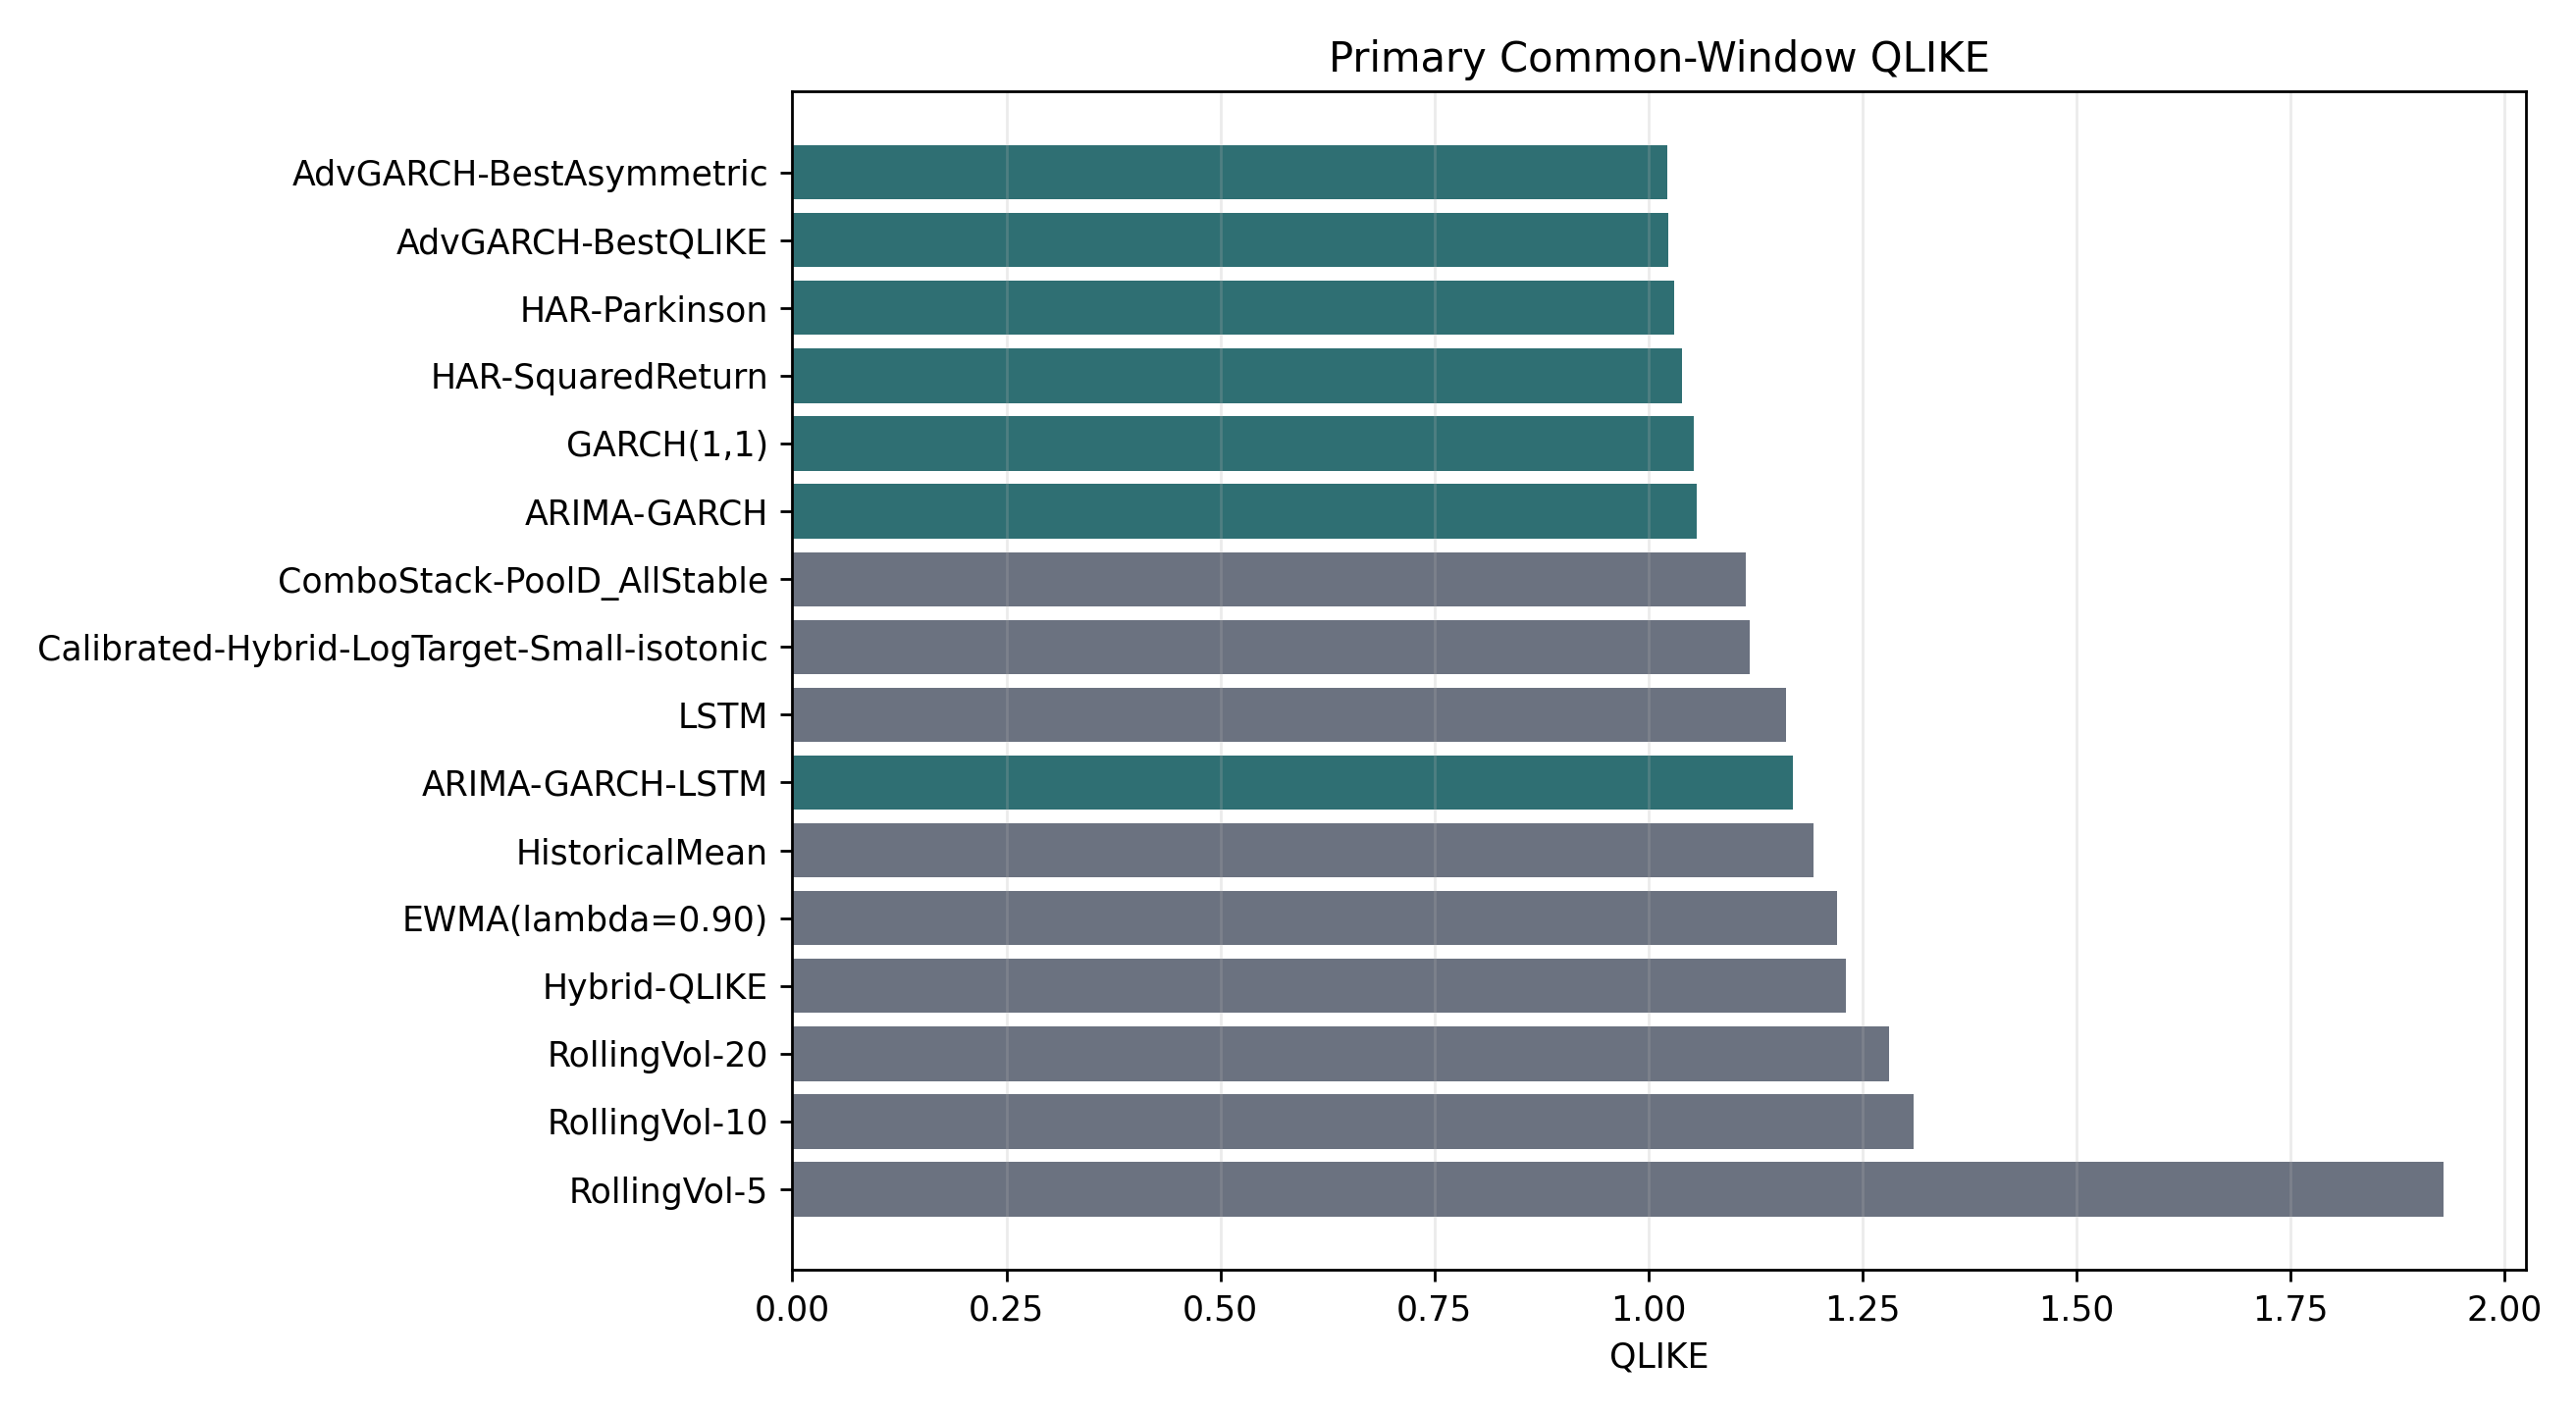
\includegraphics[width=\columnwidth]{fig_common_window_master_qlike.png}
\caption{Primary common-window QLIKE for the verified 726-observation leaderboard. Lower is better.}
\label{fig:common-window-master-qlike}
\end{figure}

\subsection{Parameter and Residual Diagnostics}

\begin{table*}[!t]
\centering
\caption{Selected GARCH-family parameter diagnostics. Persistence and half-life are reported only where the formula is technically appropriate.}
\label{tab:garch-parameter-diagnostics}
\scriptsize
\setlength{\tabcolsep}{4pt}
\begin{tabular}{@{}L{0.20\textwidth}L{0.16\textwidth}L{0.10\textwidth}rrrrL{0.13\textwidth}@{}}
\toprule
Model & Variance equation & Parameter & Estimate & Std. err. & \(p\)-value & Persistence & Validity \\
\midrule
GARCH(1,1) & GARCH(1,1) & mu & 0.0456 & 0.0204 & 0.0256 & 0.9733 & stationary \\
GARCH(1,1) & GARCH(1,1) & omega & 0.0374 & 0.0163 & 0.022 & 0.9733 & stationary \\
GARCH(1,1) & GARCH(1,1) & alpha[1] & 0.1257 & 0.0212 & 3.16e-09 & 0.9733 & stationary \\
GARCH(1,1) & GARCH(1,1) & beta[1] & 0.8476 & 0.0303 & 1.61e-172 & 0.9733 & stationary \\
AdvGARCH-BestQLIKE & EGARCH(1,1,2) & omega & 0.0063 & 0.0057 & 0.273 & 0.9503 & EGARCH persist. \\
AdvGARCH-BestQLIKE & EGARCH(1,1,2) & alpha[1] & 0.2380 & 0.0271 & 1.84e-18 & 0.9503 & EGARCH persist. \\
AdvGARCH-BestQLIKE & EGARCH(1,1,2) & gamma[1] & -0.0440 & 0.0186 & 0.0178 & 0.9503 & EGARCH persist. \\
AdvGARCH-BestQLIKE & EGARCH(1,1,2) & beta[1] & 0.9503 & 0.1492 & 1.91e-10 & 0.9503 & EGARCH persist. \\
AdvGARCH-BestQLIKE & EGARCH(1,1,2) & beta[2] & 0.0000 & 0.1536 & 1 & 0.9503 & EGARCH persist. \\
AdvGARCH-BestAsymmetric & EGARCH(1,1,1) & omega & 0.0088 & 0.0056 & 0.116 & 0.9532 & EGARCH persist. \\
AdvGARCH-BestAsymmetric & EGARCH(1,1,1) & alpha[1] & 0.2353 & 0.0283 & 1e-16 & 0.9532 & EGARCH persist. \\
AdvGARCH-BestAsymmetric & EGARCH(1,1,1) & gamma[1] & -0.0430 & 0.0189 & 0.0228 & 0.9532 & EGARCH persist. \\
AdvGARCH-BestAsymmetric & EGARCH(1,1,1) & beta[1] & 0.9532 & 0.0139 & 0 & 0.9532 & EGARCH persist. \\
\bottomrule
\end{tabular}
\end{table*}


Table~\ref{tab:garch-parameter-diagnostics} gives the post-estimation financial econometric diagnostics. For GARCH(1,1), \(\alpha=0.1257\), \(\beta=0.8476\), and \(\alpha+\beta=0.9733\). The persistence is below one, so the unconditional variance and shock half-life are technically defined; the estimated half-life is about 25.6 trading days. This supports the economic interpretation that volatility shocks to the VN-Index decay slowly.

The two EGARCH specifications also display high log-variance persistence, with beta-sum measures near 0.95. Both AdvGARCH-BestQLIKE and AdvGARCH-BestAsymmetric have negative and statistically significant \(\gamma[1]\) estimates at conventional levels. Under the EGARCH sign convention, this is consistent with negative shocks raising future volatility more than positive shocks of comparable standardized magnitude. The evidence supports an asymmetric volatility response, but it should still be read cautiously because the models are selected from a broad specification search.

\begin{table*}[!t]
\centering
\caption{Post-fit residual diagnostics for selected GARCH-family models.}
\label{tab:garch-residual-diagnostics}
\scriptsize
\begin{tabular}{@{}L{0.20\textwidth}L{0.10\textwidth}L{0.19\textwidth}rrrr@{}}
\toprule
Model & Test & Series & Lag & Statistic & \(p\)-value & Flag \\
\midrule
GARCH(1,1) & Ljung-Box & Squared std. resid. & 5 & 1.283 & 0.937 & not\_rejected \\
GARCH(1,1) & Ljung-Box & Squared std. resid. & 10 & 3.417 & 0.97 & not\_rejected \\
GARCH(1,1) & Ljung-Box & Squared std. resid. & 20 & 14.273 & 0.816 & not\_rejected \\
GARCH(1,1) & ARCH-LM & Std. resid. & 5 & 1.267 & 0.938 & not\_rejected \\
GARCH(1,1) & ARCH-LM & Std. resid. & 10 & 3.357 & 0.972 & not\_rejected \\
GARCH(1,1) & ARCH-LM & Std. resid. & 20 & 13.936 & 0.834 & not\_rejected \\
AdvGARCH-BestQLIKE & Ljung-Box & Squared std. resid. & 5 & 2.309 & 0.805 & not\_rejected \\
AdvGARCH-BestQLIKE & Ljung-Box & Squared std. resid. & 10 & 3.789 & 0.956 & not\_rejected \\
AdvGARCH-BestQLIKE & Ljung-Box & Squared std. resid. & 20 & 15.057 & 0.773 & not\_rejected \\
AdvGARCH-BestQLIKE & ARCH-LM & Std. resid. & 5 & 2.273 & 0.81 & not\_rejected \\
AdvGARCH-BestQLIKE & ARCH-LM & Std. resid. & 10 & 3.699 & 0.96 & not\_rejected \\
AdvGARCH-BestQLIKE & ARCH-LM & Std. resid. & 20 & 14.517 & 0.803 & not\_rejected \\
AdvGARCH-BestAsymmetric & Ljung-Box & Squared std. resid. & 5 & 1.938 & 0.858 & not\_rejected \\
AdvGARCH-BestAsymmetric & Ljung-Box & Squared std. resid. & 10 & 3.249 & 0.975 & not\_rejected \\
AdvGARCH-BestAsymmetric & Ljung-Box & Squared std. resid. & 20 & 15.089 & 0.771 & not\_rejected \\
AdvGARCH-BestAsymmetric & ARCH-LM & Std. resid. & 5 & 1.921 & 0.86 & not\_rejected \\
AdvGARCH-BestAsymmetric & ARCH-LM & Std. resid. & 10 & 3.213 & 0.976 & not\_rejected \\
AdvGARCH-BestAsymmetric & ARCH-LM & Std. resid. & 20 & 14.528 & 0.803 & not\_rejected \\
\bottomrule
\end{tabular}
\end{table*}


Table~\ref{tab:garch-residual-diagnostics} shows that squared standardized residual dependence is largely removed for the selected GARCH-family models. Ljung-Box tests on squared standardized residuals and ARCH-LM tests do not reject at lags 5, 10, or 20. This contrasts with the strong ARCH-LM rejections in raw returns and indicates that the models capture much of the conditional heteroskedasticity. Standardized residuals remain non-normal, however, so heavy tails and tail-risk calibration remain important.

\subsection{Statistical Comparisons}

The common-window Diebold-Mariano outputs are intentionally interpreted conservatively. Against GARCH(1,1), AdvGARCH-BestAsymmetric has a raw QLIKE comparison \(p=0.0015\) and Holm-adjusted \(p=0.0215\) within the final primary QLIKE family. AdvGARCH-BestQLIKE has raw \(p=0.0181\), but its Holm-adjusted \(p=0.2354\) does not support a decisive superiority claim after family-wise correction. HAR-Parkinson is close to GARCH(1,1), but the paired QLIKE difference is not statistically decisive. The statistical message is therefore class-level rather than single-winner: selected GARCH-family specifications and HAR-Parkinson are the strongest group.

\subsection{Rolling-Origin Refit Robustness}

\begin{table*}[!t]
\centering
\caption{Static versus expanding-window monthly refit robustness on the unified common window.}
\label{tab:refit-protocol-results}
\scriptsize
\setlength{\tabcolsep}{4pt}
\begin{tabular}{@{}L{0.18\textwidth}L{0.12\textwidth}rrrrrrrr@{}}
\toprule
Model & Protocol & \(N\) & Full & QLIKE & RMSE & MAE & Pred./Actual & Q90 QLIKE & Failed \\
\midrule
ARIMA-GARCH & expanding\_monthly & 726 & yes & 1.049005 & 3.669563 & 1.417771 & 1.049 & 6.521 & 0 \\
ARIMA-GARCH & static\_train\_only & 726 & yes & 1.055679 & 3.671816 & 1.400256 & 1.020 & 6.770 & 0 \\
AdvGARCH-BestAsymmetric & expanding\_monthly & 726 & yes & 1.014849 & 3.556510 & 1.350518 & 0.997 & 6.388 & 0 \\
AdvGARCH-BestAsymmetric & static\_train\_only & 726 & yes & 1.021413 & 3.565782 & 1.314342 & 0.933 & 6.713 & 0 \\
AdvGARCH-BestQLIKE & expanding\_monthly & 340 & no & 1.202280 & 4.350815 & 1.532191 & 0.927 & 7.762 & 19 \\
AdvGARCH-BestQLIKE & static\_train\_only & 726 & yes & 1.022898 & 3.583987 & 1.318196 & 0.931 & 6.730 & 0 \\
EWMA(lambda=0.90) & expanding\_monthly & 726 & yes & 1.219608 & 3.716363 & 1.410256 & 1.000 & 8.425 & 0 \\
EWMA(lambda=0.90) & static\_train\_only & 726 & yes & 1.219608 & 3.716363 & 1.410256 & 1.000 & 8.425 & 0 \\
GARCH(1,1) & expanding\_monthly & 726 & yes & 1.047945 & 3.656469 & 1.415344 & 1.054 & 6.523 & 0 \\
GARCH(1,1) & static\_train\_only & 726 & yes & 1.052888 & 3.648839 & 1.393909 & 1.024 & 6.766 & 0 \\
HAR-Parkinson & expanding\_monthly & 726 & yes & 1.029873 & 3.647880 & 1.374900 & 1.007 & 6.130 & 0 \\
HAR-Parkinson & static\_train\_only & 726 & yes & 1.029373 & 3.621325 & 1.353338 & 0.971 & 6.337 & 0 \\
\bottomrule
\end{tabular}
\end{table*}


Table~\ref{tab:refit-protocol-results} compares static train-only forecasts with expanding-window monthly refits for the small preselected econometric set. The conclusion largely survives. AdvGARCH-BestAsymmetric remains the best complete-window refit model, improving from static QLIKE 1.021413 to expanding-monthly QLIKE 1.014849. GARCH(1,1) improves from 1.052888 to 1.047945, and ARIMA-GARCH improves from 1.055679 to 1.049005. HAR-Parkinson remains stable, with essentially unchanged QLIKE around 1.03.

The robustness experiment also reveals operational fragility. AdvGARCH-BestQLIKE is the primary validation-selected advanced specification in the static protocol, but its monthly expanding refit fails in 19 monthly segments and only produces 340 common-window forecasts. That incomplete refit has QLIKE 1.202280 and is marked as not covering the full common window. This does not invalidate the static primary result, but it weakens the practical attractiveness of using that ARIMA-EGARCH specification in a monthly operational refit setting.

Periodic updating improves some complete econometric forecasts and reduces the one-percent common-Normal VaR violation count for several models. For example, GARCH(1,1) declines from 15 to 14 one-percent violations after monthly refitting, while AdvGARCH-BestAsymmetric declines from 14 to 13. The changes are useful but do not remove the need for tail-risk diagnostics.

\begin{figure}[!t]
\centering
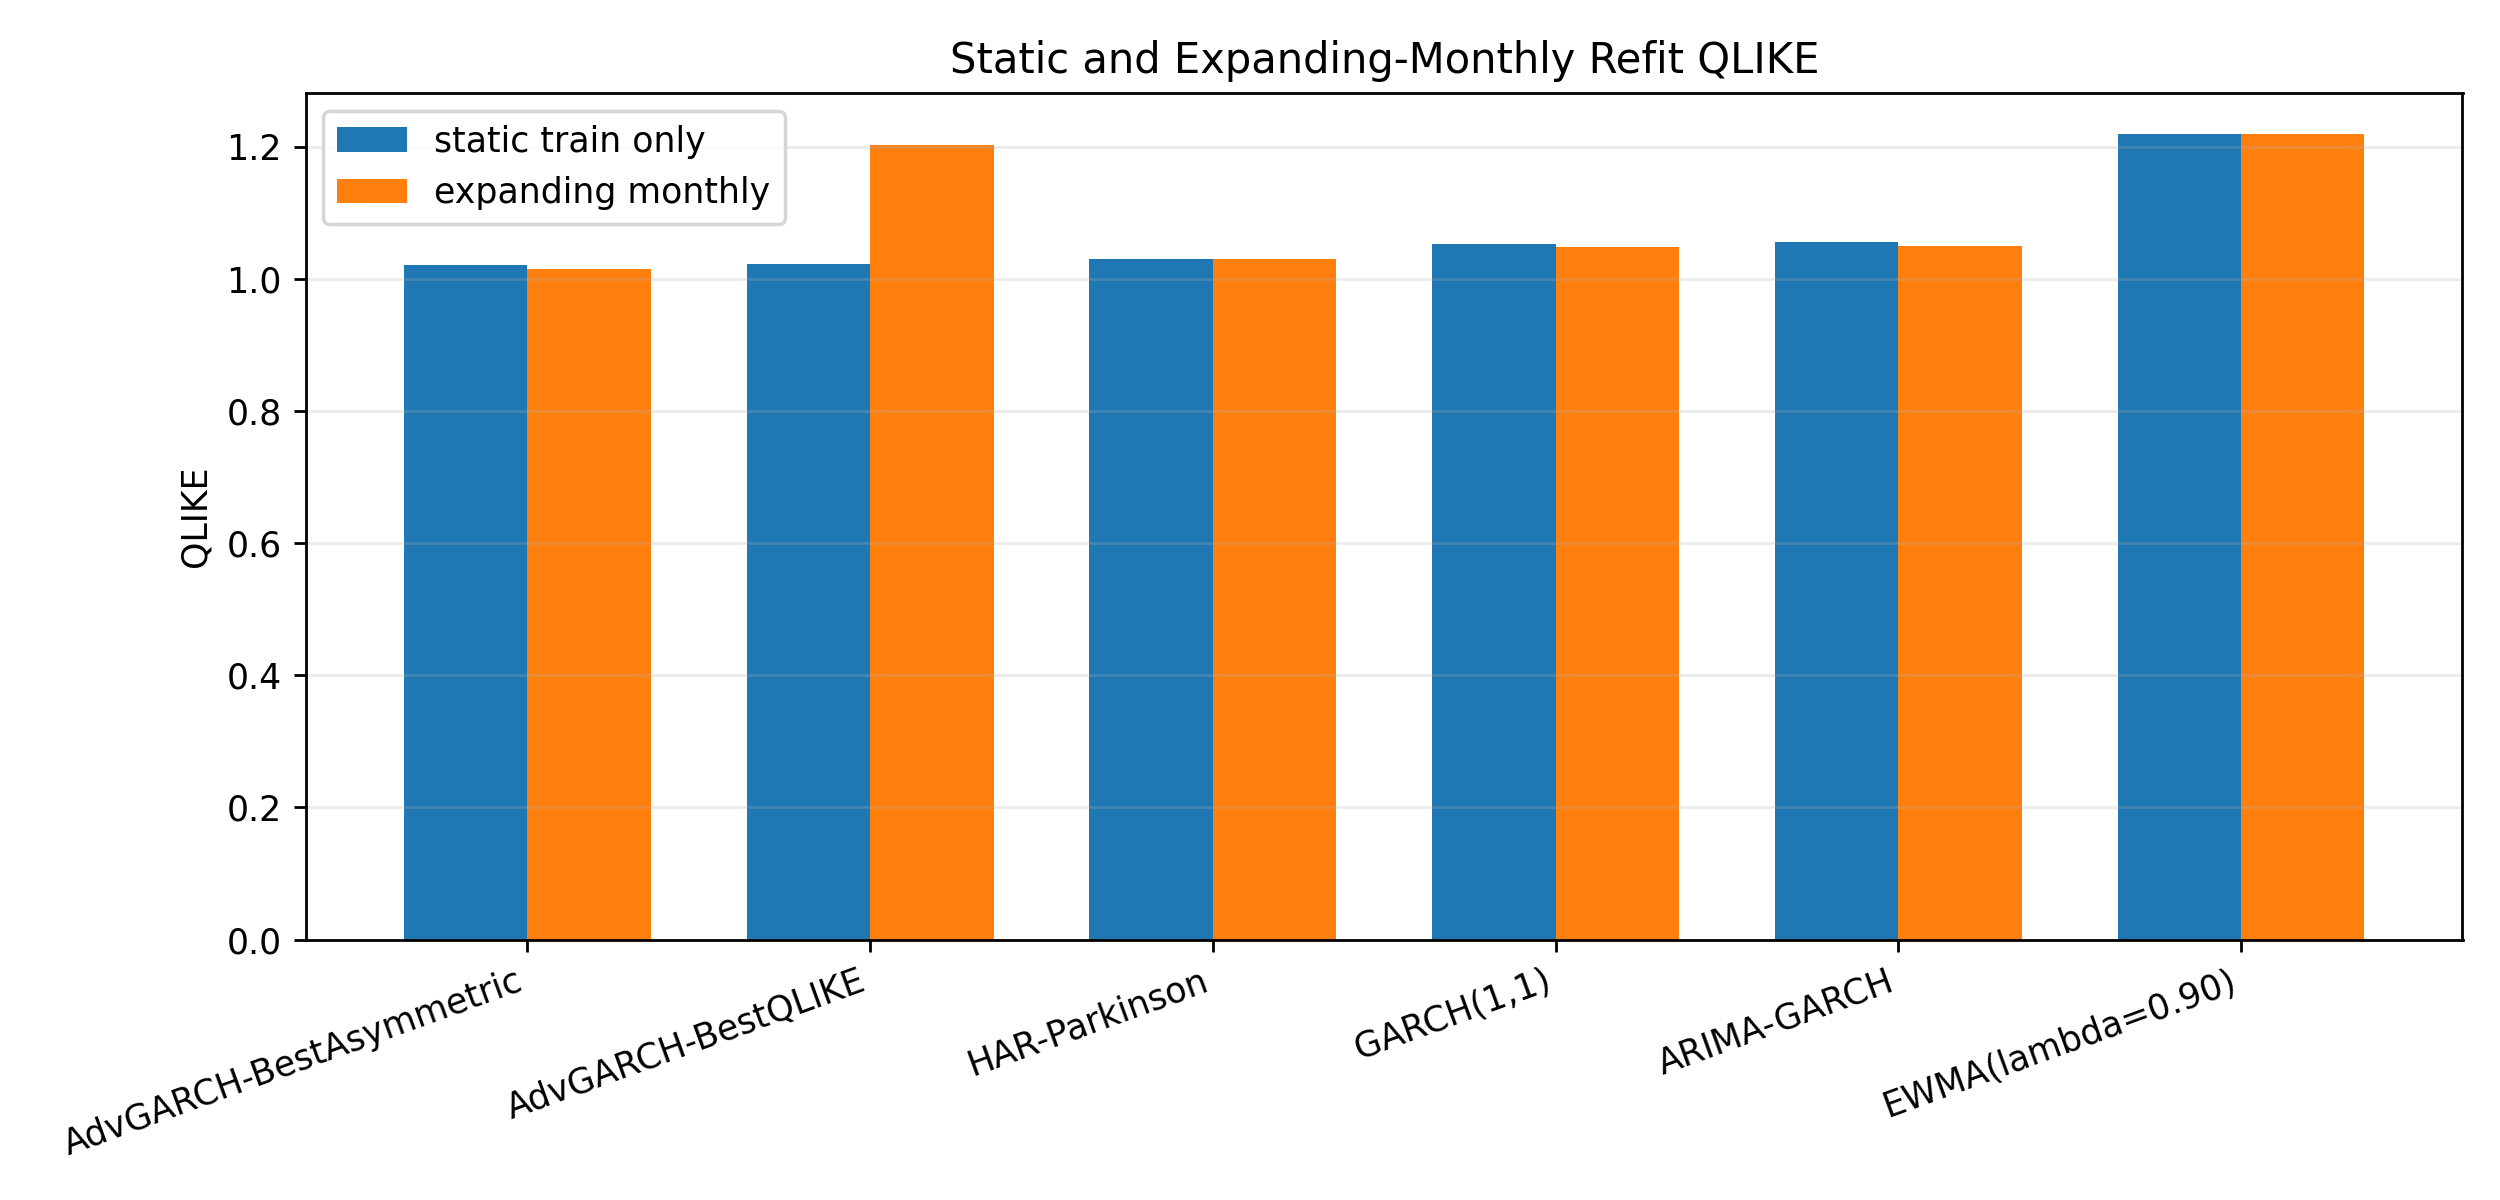
\includegraphics[width=\columnwidth]{fig_refit_protocol_qlike.png}
\caption{Static and expanding-monthly QLIKE for the controlled refit robustness experiment.}
\label{fig:refit-protocol-qlike}
\end{figure}

\subsection{Spike and VaR Diagnostics}

\begin{table*}[!t]
\centering
\caption{Common-window spike-day diagnostics at the 90th percentile of actual variance.}
\label{tab:common-window-spike-diagnostics}
\scriptsize
\begin{tabular}{@{}L{0.24\textwidth}rrrr@{}}
\toprule
Model & Spike days & Underpred. & Severe & Spike QLIKE \\
\midrule
AdvGARCH-BestAsymmetric & 73 & 97.3\% & 76.7\% & 6.713 \\
AdvGARCH-BestQLIKE & 73 & 94.5\% & 75.3\% & 6.730 \\
HAR-Parkinson & 73 & 93.2\% & 76.7\% & 6.337 \\
GARCH(1,1) & 73 & 94.5\% & 72.6\% & 6.766 \\
ARIMA-GARCH & 73 & 94.5\% & 74.0\% & 6.770 \\
EWMA(lambda=0.90) & 73 & 93.2\% & 72.6\% & 8.425 \\
LSTM & 73 & 100.0\% & 56.2\% & 5.099 \\
ARIMA-GARCH-LSTM & 73 & 100.0\% & 56.2\% & 4.793 \\
\bottomrule
\end{tabular}
\end{table*}


Average QLIKE hides a common risk weakness. Table~\ref{tab:common-window-spike-diagnostics} evaluates days above the 90th percentile of actual variance. The strongest econometric models still underpredict most spike days, and severe underprediction rates remain high. HAR-Parkinson has the best spike-day QLIKE among the primary econometric models in the table, but it still severely underpredicts about three quarters of spike days. Spike diagnostics therefore qualify rather than overturn the average-loss ranking.

\begin{table}[!t]
\centering
\caption{Common-window common-Normal VaR backtests.}
\label{tab:common-window-var-backtests}
\scriptsize
\begin{tabular}{@{}L{0.38\columnwidth}rrrrr@{}}
\toprule
Model & Level & \(N\) & Viol. & Expected & Kupiec \(p\) \\
\midrule
AdvGARCH-BestAsymmetric & 5\% & 726 & 33 & 36.30 & 0.568 \\
AdvGARCH-BestAsymmetric & 1\% & 726 & 14 & 7.26 & 0.0258 \\
AdvGARCH-BestQLIKE & 5\% & 726 & 33 & 36.30 & 0.568 \\
AdvGARCH-BestQLIKE & 1\% & 726 & 14 & 7.26 & 0.0258 \\
HAR-Parkinson & 5\% & 726 & 32 & 36.30 & 0.455 \\
HAR-Parkinson & 1\% & 726 & 15 & 7.26 & 0.0116 \\
GARCH(1,1) & 5\% & 726 & 34 & 36.30 & 0.692 \\
GARCH(1,1) & 1\% & 726 & 15 & 7.26 & 0.0116 \\
ARIMA-GARCH & 5\% & 726 & 34 & 36.30 & 0.692 \\
ARIMA-GARCH & 1\% & 726 & 15 & 7.26 & 0.0116 \\
EWMA(lambda=0.90) & 5\% & 726 & 37 & 36.30 & 0.905 \\
EWMA(lambda=0.90) & 1\% & 726 & 17 & 7.26 & 0.00197 \\
\bottomrule
\end{tabular}
\end{table}


Table~\ref{tab:common-window-var-backtests} maps variance forecasts to VaR using a common Normal quantile. At the 5\% level, the main econometric models have violation counts near expectation. At the 1\% level, strict-tail coverage is weaker. GARCH(1,1) has 15 violations out of 726 observations against 7.26 expected, with Kupiec \(p=0.0116\). AdvGARCH-BestQLIKE and AdvGARCH-BestAsymmetric each have 14 violations, with Kupiec \(p=0.0258\). These results show that good average volatility forecasts do not automatically deliver adequate extreme-risk calibration under the common-Normal mapping.

This is a standardized risk translation, not a full distribution-specific VaR evaluation. Heavy-tailed or skewed GARCH models may require model-specific quantiles, but the current primary prediction artifacts do not retain all fitted tail-shape and skew parameters needed for a clean distribution-specific comparison.

\subsection{Proxy Robustness}

\begin{figure}[!t]
\centering
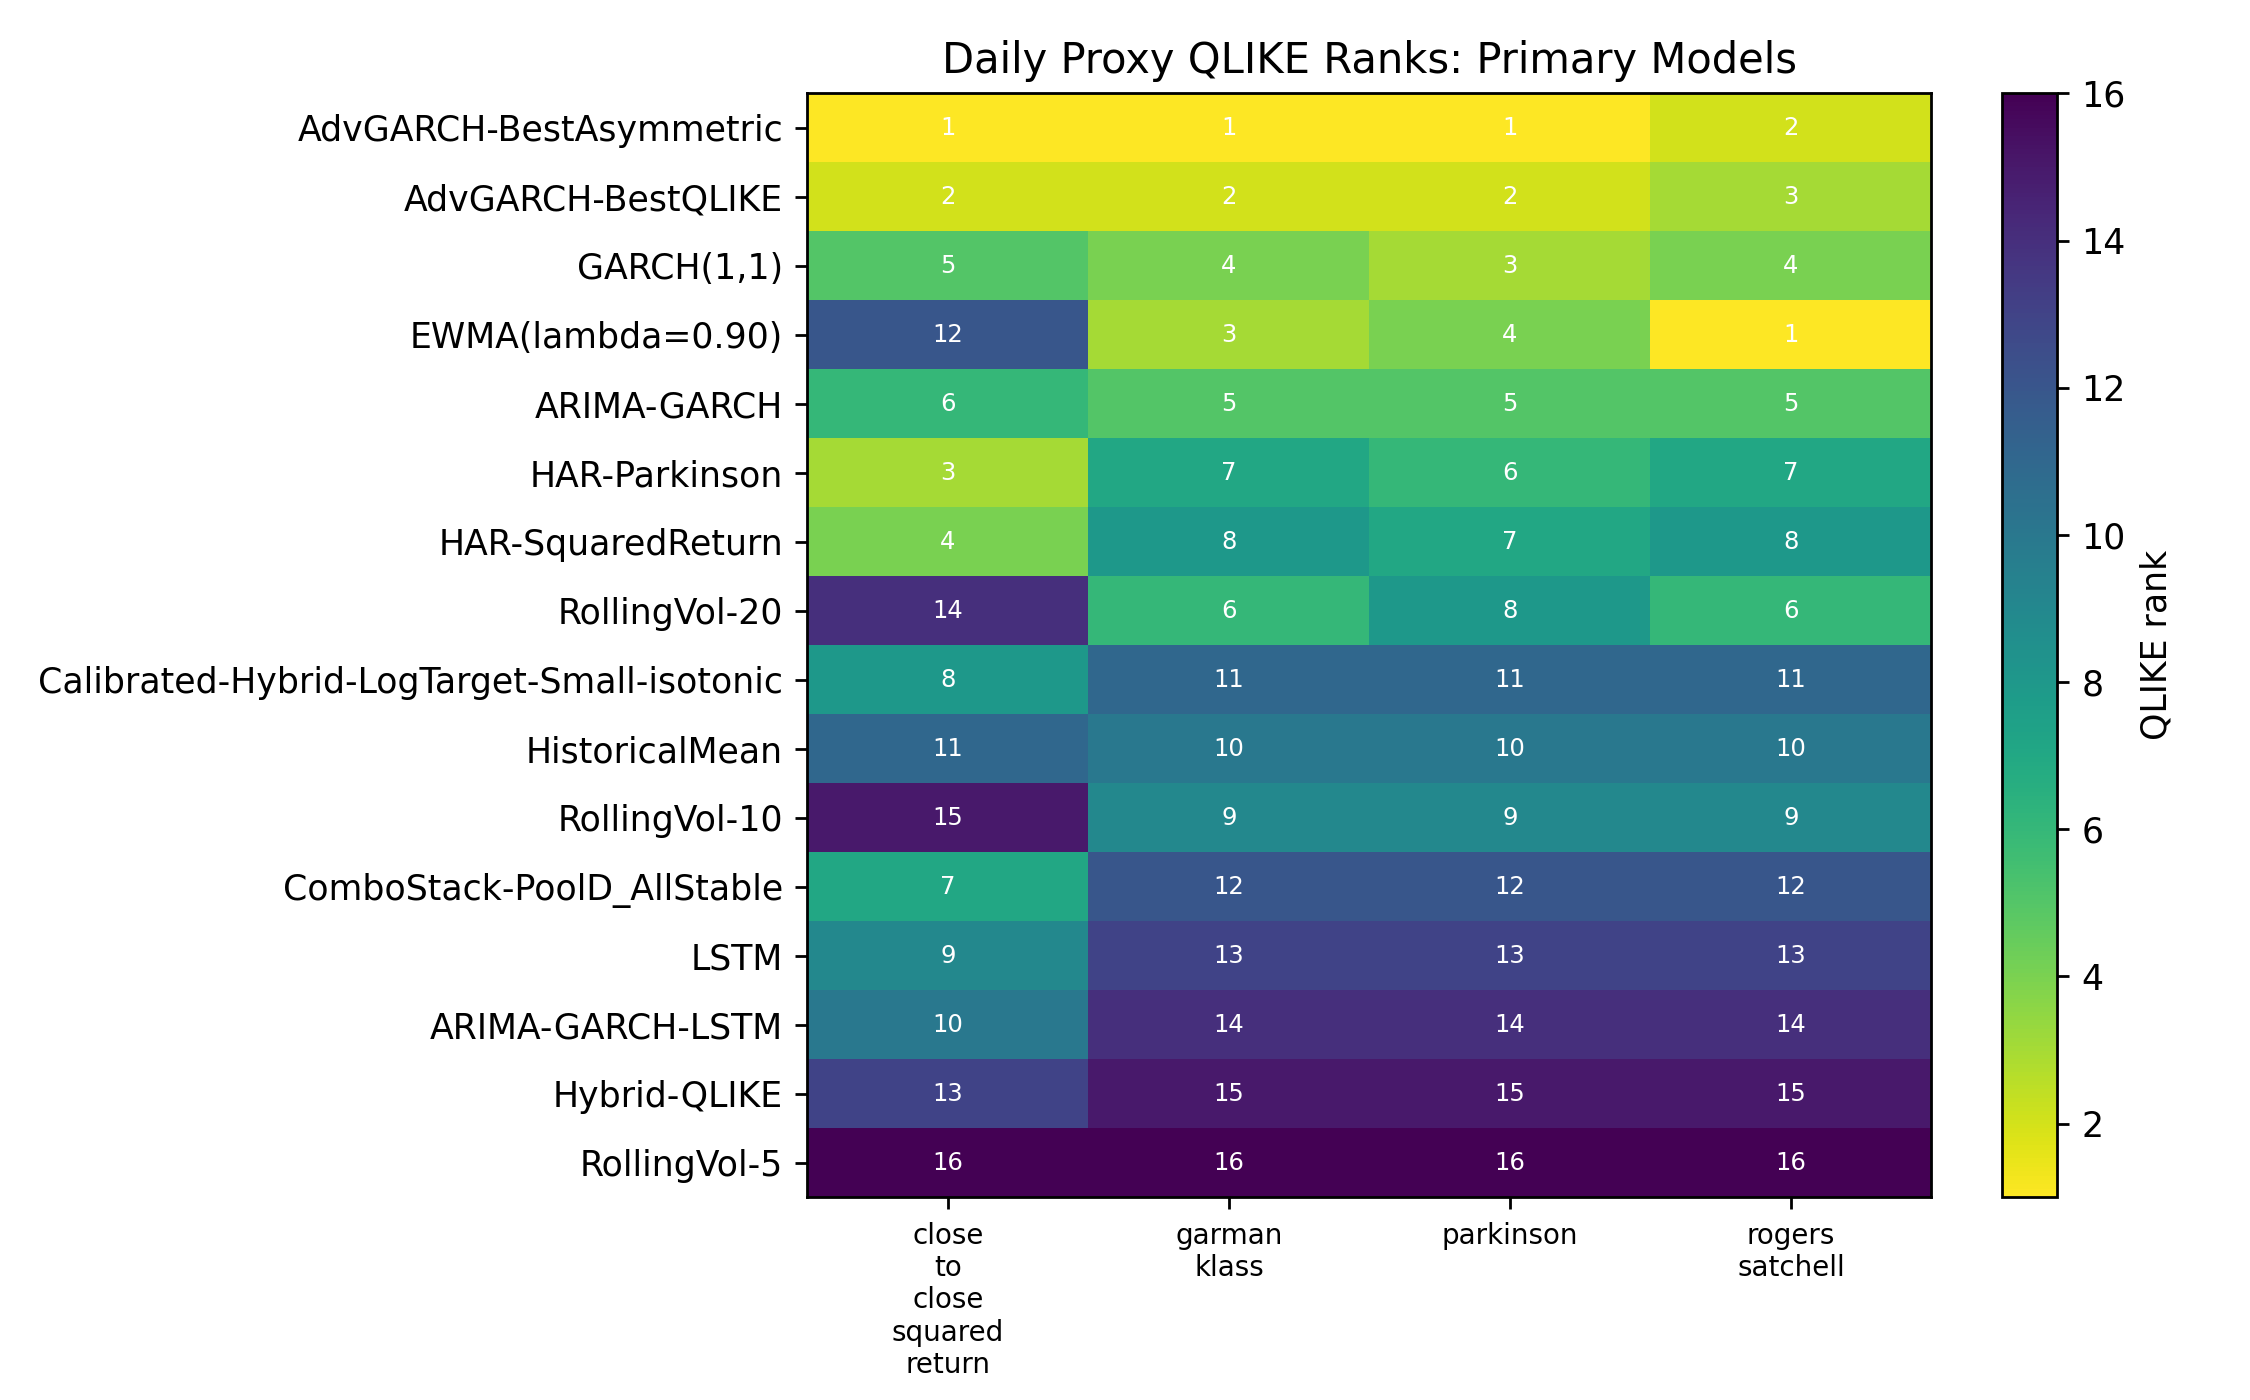
\includegraphics[width=\columnwidth]{fig_daily_proxy_rank_heatmap_primary.png}
\caption{Daily same-horizon proxy robustness for primary models. Numbers are QLIKE ranks; lower ranks are better.}
\label{fig:daily-proxy-rank-heatmap}
\end{figure}

The proxy robustness exercise confirms that exact rankings are sensitive to how latent volatility is observed. Daily close-to-close, Parkinson, Garman-Klass, and Rogers-Satchell proxies measure related but non-identical volatility objects. The main conclusion remains class-level: GARCH-family specifications are consistently competitive, and HAR-Parkinson is strong on the squared-return target because it uses OHLC range information directly. Rolling Yang-Zhang sensitivities are kept separate because they are smoothed, overlapping measurements rather than direct one-day targets.

\subsection{Discussion}

The empirical findings are economically coherent. Raw VN-Index returns are heavy-tailed and negatively skewed, while squared returns exhibit strong dependence. GARCH-family models perform well because they encode this persistence directly. HAR-Parkinson performs competitively because daily range information carries volatility information that close-to-close squared returns alone may miss.

The neural and hybrid findings are best interpreted as modest and dataset-specific. Daily sample size is limited for deep sequence models, and smooth neural forecasts can look acceptable under some average losses while missing spike timing or tail risk. Calibration and combinations can improve scale, but the implemented neural and hybrid approaches do not provide robust superiority over the strongest econometric benchmarks.

\section{Limitations}

The study uses daily data only and lacks high-frequency realized volatility. Squared returns and OHLC range estimators are imperfect proxies for latent volatility, so proxy robustness is informative but not a substitute for realized-variance targets.

The advanced GARCH search is broad and numerically fragile. Although the static validation-selected models are useful, the refit experiment shows that AdvGARCH-BestQLIKE is not operationally stable under monthly expanding refits. The asymmetric comparator performs well, but it remains a category-selected robustness model rather than the sole primary winner.

Distribution-specific VaR is not implemented in the final evidence because the prediction artifacts do not cleanly retain all innovation distribution parameters. Neural sequence construction has been corrected in code, but full retraining into versioned output paths was not performed in the final pass. This does not affect the fairness of the primary leaderboard, because all primary models are compared on the same 726 target dates.

\section{Discussion}

The results are consistent with the structure of daily equity-index volatility. GARCH-family models directly encode volatility persistence, and the fitted persistence values near 0.97 indicate that this structure is empirically important for the VN-Index. ARIMA mean filtering adds little because the conditional mean of daily returns is small relative to the variance process, so the residual-volatility forecast is close to direct GARCH.

Asymmetric and EGARCH-type variants are favored by the advanced search and by range-based proxy robustness. This is plausible for equity-index returns because negative and positive shocks can have different implications for subsequent risk, and EGARCH specifications can represent asymmetric variance responses without the same positivity constraints as standard GARCH. The evidence is strongest as a robustness pattern rather than as a Holm-corrected declaration of one superior model.

The neural results illustrate a metric trade-off. LSTM and hybrid models are not dismissed: calibrated neural forecasts and pairwise combinations show that nonlinear or hybrid signals can contain information. The issue is reliability under volatility-specific evaluation. Log-target variants can reduce MAE by producing low smooth forecasts, but QLIKE, underprediction analysis, and VaR backtests show that this behavior can miss spikes and understate risk. Calibration reduces scale bias, yet it does not fully solve timing and shape errors.

Volatility proxy choice matters. Squared daily return, Parkinson, Garman-Klass, Rogers-Satchell, and Yang-Zhang proxies do not measure identical objects. The ranking changes under smoother range-based proxies, while class-level conclusions remain broadly stable: GARCH-family forecasts are strongest, asymmetric variants are most robust, and pure neural or hybrid models do not consistently dominate.

\section{Limitations}

Several limitations qualify the findings. The study uses daily data only; high-frequency realized volatility is not available. Squared returns and OHLC range estimators are proxies for latent volatility rather than true volatility. The advanced GARCH-family search is broad enough to create validation-overfitting risk, and 576 candidate fits fail numerically. The MCS is a documented moving-block bootstrap approximation and retains many models, so it should be read as conservative evidence against a decisive winner.

The neural models are trained on a modest daily sample for deep learning. Test results cover 2023--2025 and may reflect regime-specific market conditions. Forecast combinations and ex-post best test models are useful diagnostics, but they should not be interpreted as primary selected winners. Finally, all VaR forecasts use a common Normal-quantile mapping, which standardizes comparison but does not exploit distribution-specific tail parameters from fitted GARCH-family models.

\section{Conclusion}

This paper provides a robust empirical benchmark for one-step-ahead VN-Index volatility forecasting under validation-based selection, statistical testing, risk backtesting, and volatility-proxy robustness. The main conclusion is that GARCH-family models remain the most reliable class for daily VN-Index volatility forecasting. GARCH(1,1) is a competitive and well-calibrated benchmark, while broader GARCH-family search and OHLC proxy analysis favor asymmetric or EGARCH-type specifications.

ARIMA mean dynamics add limited standalone value. Neural and hybrid models do not robustly dominate econometric benchmarks, although calibrated neural forecasts and selected combinations suggest that hybrid information can be complementary. Log-target neural variants can reduce MAE, but they systematically underpredict volatility spikes and substantially understate tail risk before calibration. The evidence also shows that volatility proxy choice matters: directional conclusions are stable, but exact rankings are not invariant across squared-return and range-based targets.

For applied VN-Index risk forecasting, the practical implication is conservative. Use GARCH-family forecasts as the benchmark class, treat advanced asymmetric specifications as robust candidates, evaluate neural and hybrid forecasts with volatility-specific losses rather than MAE alone, and validate conclusions under alternative volatility proxies and risk backtests before using them for risk management.


\bibliographystyle{IEEEtran}
\bibliography{references}

\end{document}
